\def\leftcircle{(-1,0) circle (2 cm)}
\def\rightcircle{(1,0) circle (2 cm)}

\begin{figure}[H]
  \centering
  \label{tikzpic:set_minus}
  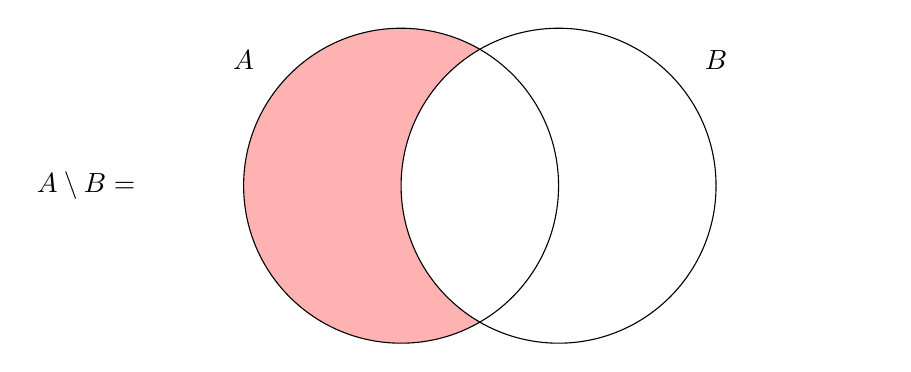
\begin{tikzpicture}
    \begin{scope}
      \clip \rightcircle (-3,-2) rectangle (3,2);;
      \fill[red!30] \leftcircle;
    \end{scope}
    
      \draw \leftcircle;
      \draw \rightcircle;
      \draw (-3,1.6) node {$A$};
      \draw (3,1.6) node {$B$};
      \draw (-5,0) node {$A \setminus B = $};
      \draw (5,0) node {\text{     }};
  \end{tikzpicture}
  \caption{Разность множеств}
\end{figure}

